\documentclass{article}

\usepackage{fancyhdr}
\usepackage{extramarks}
\usepackage{amsmath}
\usepackage{amsthm}
\usepackage{amsfonts}
\usepackage{tikz}
\usepackage[plain]{algorithm}
\usepackage{algpseudocode}

\usetikzlibrary{automata,positioning}

%
% Basic Document Settings
%

\topmargin=-0.45in
\evensidemargin=0in
\oddsidemargin=0in
\textwidth=6.5in
\textheight=9.0in
\headsep=0.25in

\linespread{1.1}

\pagestyle{fancy}
\lhead{\hmwkAuthorName}
\chead{\hmwkClass\ (\hmwkClassInstructor\ \hmwkClassTime): \hmwkTitle}
\rhead{\firstxmark}
\lfoot{\lastxmark}
\cfoot{\thepage}

\renewcommand\headrulewidth{0.4pt}
\renewcommand\footrulewidth{0.4pt}

\setlength\parindent{0pt}

%
% Create Problem Sections
%

\newcommand{\enterProblemHeader}[1]{
    \nobreak\extramarks{}{Problem \arabic{#1} continued on next page\ldots}\nobreak{}
    \nobreak\extramarks{Problem \arabic{#1} (continued)}{Problem \arabic{#1} continued on next page\ldots}\nobreak{}
}

\newcommand{\exitProblemHeader}[1]{
    \nobreak\extramarks{Problem \arabic{#1} (continued)}{Problem \arabic{#1} continued on next page\ldots}\nobreak{}
    \stepcounter{#1}
    \nobreak\extramarks{Problem \arabic{#1}}{}\nobreak{}
}

\setcounter{secnumdepth}{0}
\newcounter{partCounter}
\newcounter{homeworkProblemCounter}
\setcounter{homeworkProblemCounter}{1}
\nobreak\extramarks{Problem \arabic{homeworkProblemCounter}}{}\nobreak{}

%
% Homework Problem Environment
%
% This environment takes an optional argument. When given, it will adjust the
% problem counter. This is useful for when the problems given for your
% assignment aren't sequential. See the last 3 problems of this template for an
% example.
%
\newenvironment{homeworkProblem}[1][-1]{
    \ifnum#1>0
        \setcounter{homeworkProblemCounter}{#1}
    \fi
    \section{Problem \arabic{homeworkProblemCounter}}
    \setcounter{partCounter}{1}
    \enterProblemHeader{homeworkProblemCounter}
}{
    \exitProblemHeader{homeworkProblemCounter}
}

%
% Homework Details
%   - Title
%   - Due date
%   - Class
%   - Section/Time
%   - Instructor
%   - Author
%

\newcommand{\hmwkTitle}{Homework 4 Statics}
\newcommand{\hmwkDueDate}{April 8th, 2020}
\newcommand{\hmwkClass}{PHYS 206}
\newcommand{\hmwkClassTime}{Section 509}
\newcommand{\hmwkClassInstructor}{Dr. O}
\newcommand{\hmwkAuthorName}{\textbf{Amari West}}
\newcommand{\hmwkDueTime}{11:55pm \\ 7 Pages}

%
% Title Page
%

\title{
    \vspace{2in}
    \textmd{\textbf{\hmwkClass:\ \hmwkTitle}}\\
    \normalsize\vspace{0.1in}\small{Due\ on\ \hmwkDueDate\ at \hmwkDueTime}\\
    \vspace{0.1in}\large{\textit{\hmwkClassInstructor\ \hmwkClassTime}}
    \vspace{3in}
}

\author{\hmwkAuthorName}
\date{}

\renewcommand{\part}[1]{\textbf{\large Part \Alph{partCounter}}\stepcounter{partCounter}\\}

%
% Various Helper Commands
%

% Useful for algorithms
\newcommand{\alg}[1]{\textsc{\bfseries \footnotesize #1}}

% For derivatives
\newcommand{\deriv}[1]{\frac{\mathrm{d}}{\mathrm{d}x} (#1)}

% For partial derivatives
\newcommand{\pderiv}[2]{\frac{\partial}{\partial #1} (#2)}

% Integral dx
\newcommand{\dx}{\mathrm{d}x}

% Alias for the Solution section header
\newcommand{\solution}{\textbf{\large Solution}}

% Probability commands: Expectation, Variance, Covariance, Bias
\newcommand{\E}{\mathrm{E}}
\newcommand{\Var}{\mathrm{Var}}
\newcommand{\Cov}{\mathrm{Cov}}
\newcommand{\Bias}{\mathrm{Bias}}

% Allow double underline
\def\doubleunderline#1{\underline{\underline{#1}}}

% Allow for units in math mode
\newcommand{\unit}[1]{\ensuremath{\, \mathrm{#1}}}

\begin{document}

\maketitle

\pagebreak

\begin{homeworkProblem}
	
	A uniform in shape and mass pipe strut $BDC$ is loaded and supported as shown. The mass of the strut is $m$ kg; the acceleration due to gravity is $g \unit{m/s^2}$. The strut is supported by a smooth pin at point C and a cable at point B. There is an external force \textbf{P} (downward) at point D. The cable is light and does not stretch.
\\
	
	a) Find the unknown reaction forces (reaction at the pin and tension in the cable) in terms of given parameters like L, H, $m$, $g$, and \textbf{P}. \\
	
	b) Using the following numerical parameter values: the mass of the strut is 50 kg, the acceleration due to gravity is 9.81 $\unit{m/s^2}$, L is 0.8 m, H is 1 m, and \textbf{P} is 750 N, calculate the magnitude and direction of the force exerted by the pin on the strut at point C and the tension force in cable AB. \\
	
	\textbf{\underline{Given}}
	
	\begin{itemize}
		\item The mass of the strut, $m$.
		\item The acceleration due to gravity, $g$.
		\item Smooth pin @ point C
		\item Cable @ point B
		\item Downward force \textbf{P}
	\end{itemize}
	
	\textbf{\underline{Find}}
	\\
	
	a) The reaction forces with respect to point C.
	\\
	
	b) Using the given values to find the force at point C and the tension force in AB.
	\\
	
	\textbf{\underline{Diagram}}
	
	\includegraphics[scale=0.2]{problem1}
	
	\textbf{\underline{Theory}}
	\\
	
	To solve a problem involving statics, first assume that the net force and net moment acting on the structure is equal to 0. Use this assumption to find all of the unknown variables by solving the system of equations.
	
	\[
	\begin{split}
		\Sigma F_x &= 0
		\\
		\Sigma F_y &= 0
		\\
		\Sigma M_a &= 0
	\end{split}
	\] 
	
	\textbf{\underline{Assumptions}}
	\\
	
	a) There is no external net force acting upon the structure.
	\\
	
	b) \textbf{P} and the force of gravity are their own separate forces.
	\\
	
	\textbf{\underline{Solution}}	
	\\
	
	First, sum up all of the forces in both x and y directions along with the net moment.
	
	\[
	\begin{split}
	\Sigma F_x &= C_x - T_{AB} = 0
	\\
	\Sigma F_y &= C_y - P - mg = 0
	\\
	\Sigma M_a &= \frac{H T_{AB}}{2} + L(P + mg) = 0
	\end{split}
	\]
	
	To answer the first part of the question, solve the system for the unknowns in terms of the given parameters which yields.
	
	\[
	\begin{split}
		T_{AB} &= \frac{2(P + mg)L}{H}
		\\
		C_y &= P + mg
		\\
		C_x &= \frac{2(P + mg)L}{H}
	\end{split}
	\]
	
	To find the values for the second part, simply plug in the values.
	
	\[
	\begin{split}
		T_{AB} &= \frac{2\left(750\unit{N} + 50\unit{kg} \cdot 9.81\unit{\frac{m}{s^2}}\right)(0.8 \unit{m})}{1\unit{m}} = 1984.8 \unit{N}
		\\
		C_y &= 750\unit{N} + 50\unit{kg} \cdot 9.81\unit{\frac{m}{s^2}} = 1240.5
		\\
		C_x &= T_{AB} = 1984.8 \unit{N}
	\end{split} 
	\]
	
	Now, find the value of $\vec{C}$ and $\theta$.
	
	\[
	\begin{split}
		\vec{C} &= \sqrt{(1984.8\unit{N})^2 + (1240.5\unit{N})^2} = 2340.57\unit{N}
		\\
		\theta &= \arctan\left(\frac{1240.5}{1984.8}\right) = 32^{\circ} 
	\end{split}
	\]
	
	\textbf{\underline{Conclusion}}	
	
	\[
	\begin{split}
	T_{AB} &= 1984.8 \unit{N}
	\\
	\vec{C} &= 2340.57 \unit{N}
	\\
	\theta &= 32^{\circ}
	\end{split}
	\]
\end{homeworkProblem}

\pagebreak

\begin{homeworkProblem}
	A rectangular beam ABCDE is loaded and supported as shown. The beam has a uniform cross section and weighs 425 lbf (pound-force). There is a smooth pin at point A, a 500 lbf downward force at point B, a 250 lbf upward force at point C, a 400 lbf downward force at point D, and a smooth roller at point E. The distances between the points A, B, C, D, and E are as follows: $AB$ = 1 ft, $BC$ = 3 ft, $CD$ = 3 ft, $DE$ = 2 ft. Determine the reactions at supports A and E.
	\\
	
	\includegraphics[scale=0.2]{problem2}
	
	\textbf{\underline{Solution:}}
	
	\[
	\begin{split}
		A_y &= 607\unit{lbf}
		\\
		E_y &= 468\unit{lbf}
	\end{split}
	\]
	
\end{homeworkProblem}

\pagebreak

\begin{homeworkProblem}
	A light bar ABC is supported by a smooth pin at A and a cable at B. An external 850 N downward force is applied at point C. Determine the force exerted by the cable at point B and the reaction at support A. You may disregard the weight of the bar for the analysis. The cable is light and does not stretch.
	\\
	
	\includegraphics[scale=0.2]{problem2}
	
	\textbf{\underline{Solution:}}
	
	\[
	\begin{split}
	T_B &= -1413.58 \unit{Nmm}
	\\
	\vec{A} &= 1349.2 \unit{Nmm}
	\\
	\theta &= \arctan\left(\frac{1310.6}{320.46}\right) = 13.74^{\circ}
	\end{split}
	\]
	
	
\end{homeworkProblem}

\pagebreak

\begin{homeworkProblem}
	A weightless bar is supported by a smooth pin at A and a smooth roller at B. A 20 kN external force and a 15 kN external force act on the bar as shown. The bar is in static equilibrium. What is the external reaction at A?
	\\
	
	\textbf{\underline{Given}}
	
	\begin{itemize}
		\item Smooth pin @ point A
		\item Smooth roller @ point B
		\item The system is at static equilibrium
		\item External force of 15 kN Present
		\item External force of 20 kN Present  
	\end{itemize}
	
	\textbf{\underline{Find}}
	\\
	
	a) External Reaction at A
	\\
	
	b) Find $\unit{B_y}$ 
	
	\textbf{\underline{Diagram}}
	
	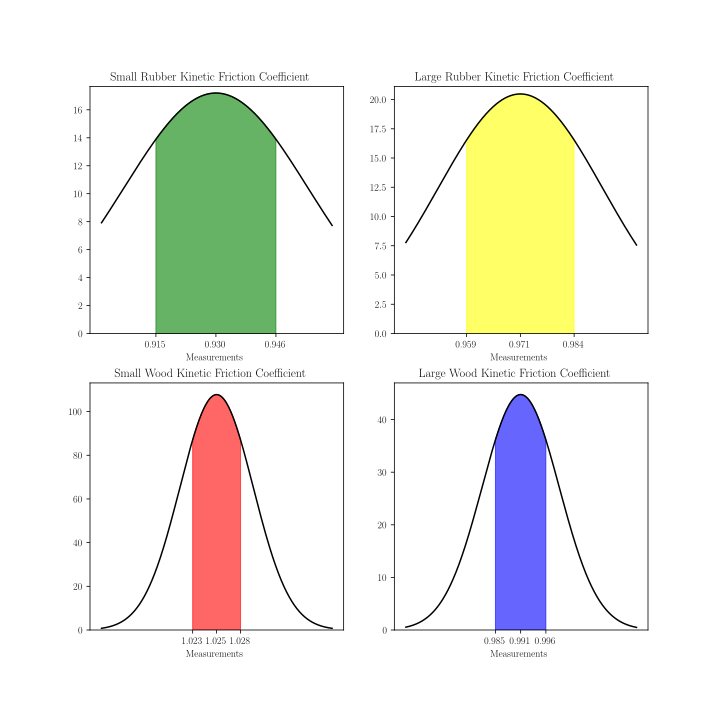
\includegraphics[scale=0.2]{problem4}
	
	\textbf{\underline{Theory}}
	\\
	
	To solve a problem involving statics, first assume that the net force and net moment acting on the structure is equal to 0. Use this assumption to find all of the unknown variables by solving the system of equations.
	
	\[
	\begin{split}
	\Sigma F_x &= 0
	\\
	\Sigma F_y &= 0
	\\
	\Sigma M_a &= 0
	\end{split}
	\] 
	
	\textbf{\underline{Assumptions}}
	\\
	
	a) The net force is equal to 0
	\\ 
	
	\textbf{\underline{Solution}}	
	\\
	
	First, to ease the burden of further calculations, find the components of the 15kN force.
	
	\[
	\begin{split}
		x: 15\unit{kN} \cdot \cos{\theta} &= 15\unit{kN} \cdot \frac{4}{5} = 12\unit{kN}
		\\
		y: 15\unit{kN} \cdot \sin{\theta} &= 15\unit{kN} \cdot \frac{3}{5} = 9\unit{kN}
	\end{split}
	\]
	
	Now, sum up all of the forces in both x and y directions along with the net moment.
	
	\[
	\begin{split}
		\Sigma F_x &= 12\unit{kN} + A_x = 0
		\\
		\Sigma F_y &= A_y - 20\unit{kN} + B_y + 9\unit{kN} = 0
		\\
		\Sigma M_A &= -20\unit{kN} \cdot 2\unit{m} + B_y \cdot 4\unit{m} + 9\unit{kN} \cdot 6\unit{m} + 12\unit{kN} \cdot 2\unit{m} = 0
	\end{split}
	\]
	
	Solve for the unknowns.
	
	\[
	\begin{split}
		B_y &= -9.5\unit{kN}
		\\
		A_x &= -12\unit{kN}
		\\
		A_y &= 20.5\unit{kN}
	\end{split}
	\]
	
	Now find the magnitude of $\vec{A}$ and $\theta$.
	
	\[
	\begin{split}
		\vec{A} &= \sqrt{(-12)^2 + (20.5)^2} = 23.75\unit{kN}
		\\
		\theta &= \arctan\left(\frac{20.5}{-12}\right) = -59.65^{\circ}
	\end{split}
	\] 
	\textbf{\underline{Conclusion}}
	\\	
	
	$\vec{A}$ = 23.75 kN @ $59.65^{\circ}$ CW
	
\end{homeworkProblem}

\pagebreak

\end{document}
